\begin{frame}{multiple APs, one network}
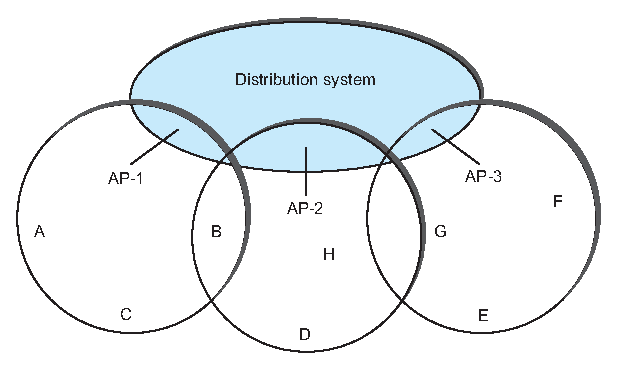
\includegraphics[width=\textwidth]{../multiaccess/cnsp-fig48}
\imagecredit{Computer Networks: A Systems Approach, figure 48}
\end{frame}

\begin{frame}{APs as switches}
    \begin{itemize}
    \item multiple APs can act as \textit{one network}
    \item example: nodes connected to different APs can send packets to each other by MAC address
    \vspace{.5cm}
    \item distribution system needs to share neighbor-table-like information
    \end{itemize}
\end{frame}

\begin{frame}{switching APs}
    \begin{itemize}
    \item nodes can switch APs\ldots
    \vspace{.5cm}
    \item check for new APs when signal strength too low
    \item periodically check for beacons + signal strength
    \vspace{.5cm}
    \item switching APs = same as joining network, but\ldots
        \begin{itemize}
        \item can keep IP address, etc.
        \item maybe optimizations to avoid redoing wifi security, etc.
        \end{itemize}
    \end{itemize}
\end{frame}

